\documentclass[paper=a4, fontsize=11pt]{scrartcl}
\usepackage[T1]{fontenc}
\usepackage{fourier}

\usepackage[english]{babel}                             % English language/hyphenation
\usepackage[protrusion=true,expansion=true]{microtype}  
\usepackage{amsmath,amsfonts,amsthm} % Math packages
\usepackage[pdftex]{graphicx} 
\usepackage{url}
\usepackage[section]{placeins}


%%% Custom sectioning
\usepackage{sectsty}
\allsectionsfont{\centering \normalfont\scshape}
\usepackage{color}
\usepackage{color,soul}

%%% Custom headers/footers (fancyhdr package)
\usepackage{fancyhdr}
\pagestyle{fancyplain}
\fancyhead{}                      % No page header
\fancyfoot[L]{}                     % Empty 
\fancyfoot[C]{}                     % Empty
\fancyfoot[R]{\thepage}                 % Pagenumbering
\renewcommand{\headrulewidth}{0pt}      % Remove header underlines
\renewcommand{\footrulewidth}{0pt}        % Remove footer underlines
\setlength{\headheight}{13.6pt}


%%% Equation and float numbering
\numberwithin{equation}{section}    % Equationnumbering: section.eq#
\numberwithin{figure}{section}      % Figurenumbering: section.fig#
\numberwithin{table}{section}       % Tablenumbering: section.tab#


%%% Maketitle metadata
\newcommand{\horrule}[1]{\rule{\linewidth}{#1}}   % Horizontal rule

\title{
    %\vspace{-1in}  
    \usefont{OT1}{bch}{b}{n}
    \normalfont \normalsize \textsc{Carnegie Mellon University - Computational Biology Department} \\ [25pt]
    \horrule{0.5pt} \\[0.4cm]
    \huge Active Learning for Drug Selection\\ on Identified Target Protein \\
    \horrule{2pt} \\[0.5cm]
}
\author{
  Christine Baek\\
  \normalsize\texttt{christib@andrew.cmu.edu}
  \and
  Qi Chu\\
  \normalsize\texttt{qchu@andrew.cmu.edu}
  \date{}
}
\date{}


\newcommand{\TODO}[1]{\textcolor{red}{\textbf{TODO: } #1}}

%%% Equation and float numbering
\numberwithin{equation}{section}    % Equationnumbering: section.eq#
\numberwithin{figure}{section}      % Figurenumbering: section.fig#
\numberwithin{table}{section}       % Tablenumbering: section.tab#
\usepackage[T1]{fontenc}
\usepackage[utf8]{inputenc}
\usepackage{tabularx,ragged2e,booktabs,caption}
\newcolumntype{C}[1]{>{\Centering}m{#1}}
\renewcommand\tabularxcolumn[1]{C{#1}}







%%% Begin document
\begin{document}
\maketitle
\section{Introduction}
In this project, we explore three datasets of different noise and/or labels, for identification of compounds that bind to specific target protein. We first perform feature selection using $\chi^2$ test, then adopt the \textit{largest positive score}~\cite{ref:warmuth} for active learning strategy, and SVM for model learning. We also perform a gradient experiment to learn the optimal balance for allocating queries between feature selection and model learning.



\section{Methods}

Input :
\begin{itemize}
\item Training data consists of 4000 training instances, each with 1000 features and true label 
\item Test data consists of 1000 testing instances, each with 1000 features and true label
\item Blind prediction data consists of 1000 instances, each with 1000 features
\item Each data(row) represents potential compound that may bind to the target
\item Each feature(column) represents a structural or chemical feature
\end{itemize}




As with real world drug target screening, we began with assumption that only an extremely small fraction of compounds will bind to the target. Also, only a small fraction of the features would be relevant in predicting the label (are actual sites that the drug can potentially bind to). Our challenge is to first find which features are relevant in accurately predicting whether the compound will bind to the target or not, and then learning on those features.


We performed a gradient experiment, and measured the performance based on the number of queries made between initial learning and active learning, as the total number of queries is capped at 2500. Our predictions are then compared against random learner, as well as 0-guess, which predicts inactivity (label=0) for all compounds. 


\subsection{Learning Strategy}

Because of the imbalanced dataset (only small portion of the molecules actually bind to target), it would have been dangerous to use active learning strategy without any prior. We decided to split our learning into two different phases : Initial and Active. During initial learning, we randomly select molecules without any assumptions or selection criteria, other than choosing molecules we have not seen before. We perform feature selection during this phase using $\chi^2$ test. Once initial learning is over, we begin the active learning phase where points are selected per \textit{largest positive score} strategy as discussed in ~\cite{ref:warmuth}, elaborated below. Total number of queries made during both initial and active phase total 2500, the allotted budget. 


\subsubsection{Initial Feature Selection}

Randomly chosen molecules are queried for their label and features. This initial phase is important in learning which features are relevant, in order to build a more relevant model. While data has been omitted, our previous attempts without explicit feature selection has returned low F1 scores as well as high error rates. For each feature, $\chi^2$ test was performed along with the true label, and we selected top 25 features to learn on. We chose feature selection but not Principle Component Analysis (PCA) for dimension reduction because of the domain knowledge that only a small number of features are important. Selecting a feature rather than a principle component also produces more meaningful result in the domain. The importance of each domain can be useful for the study.

\subsubsection{Active Compound Selection}

We used selection strategy of \textit{largest positive score} which performed the best in ~\cite{ref:warmuth}. \textit{Largest positive score} compound is selected by computing a probability of a compound to be positive. Given that most compounds are inactive and would be predicted to be 0, this strategy searches for the compounds that are predicted to be active with highest probability. We used the probability functionality of \textit{SVC} in sklearn package, which calculates the probability using 5-fold cross validation. Doing so narrows our hypothesis space, by focusing our search in the most likely regions of the hypothesis space. Given our goal of drug discovery for our target, false positives (drugs that are classified as binding to target, but does not) can be tolerated within reason, but false negatives are potentially costly. We do not expend our limited number of queries for looking up inactive compounds, but instead dedicate our efforts towards finding potentially active compounds which are few and far between. We confirm their label, or activity via query to the oracle. Note that this strategy works for our purpose of finding as many positive molecules that bind to drug target, but a different strategy such as choosing compounds near boundary may be more suited for studying the structure-activity relationship ~\cite{ref:warmuth}.

\subsection{Classifier Strategy}

Support Vector Machine (SVM) was chosen as our classifier for multiple reasons. SVM finds a hyperplane that maximizes the distance between the nearest data (support vectors) and the hyperplane. Given the high dimension of our input data (1000 features), it was important that we choose a classifier that behaves well in a high-dimension feature space. SVM separates inactive from active compounds by using maximum margin hyperplane for decision boundary.  
Gaussian kernel (default) was used for training. The kernel is computed between samples rather than in the feature space so we expect SVM to be robust when only a small number of features are relevant.
Other classifiers such as random forest and winnow were also tested but did not produce comparable results.


\section{Results}

A gradient experiment was performed for varying number of queries divided between the initial learning (feature selection) and active learning (model learning). Figures for each section (difficulty) include the best performing division of queries for each data set, but full data is available in Table~\ref{f1table} for F1 score, and Table~\ref{errortable} for error rates. For all figures below, only the queries to the oracle during active learning is included (ex: if number of queries begin at 2000, it indicates 2000 queries have already been spent on feature selection). The difference between the starting point of active learner and random learner can be explained by the random number generator since we randomly selected a same number of samples for each active learner and the companion random learner and chose to seed the random generator once with seed 0 to make it possible to reproduce the data easily. The difference does not affect our conclusions.

\subsection{Easy}


\begin{figure}[!htb]
  \centering
  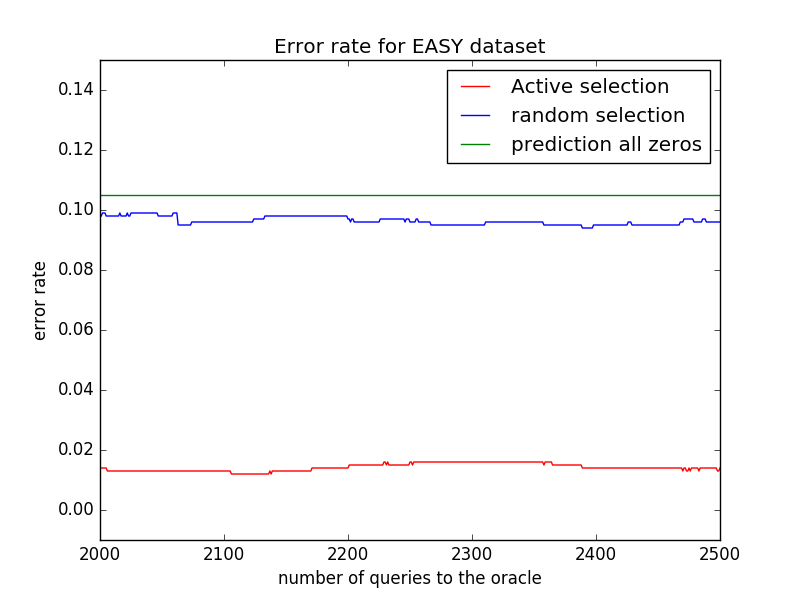
\includegraphics[scale = 0.5]{figures/error_easy.png}
      \caption{Error rate of easy data set plotted against number of queries made to oracle.}
      \label{easyerror}
\end{figure}


\begin{figure}[!htb]
  \centering
  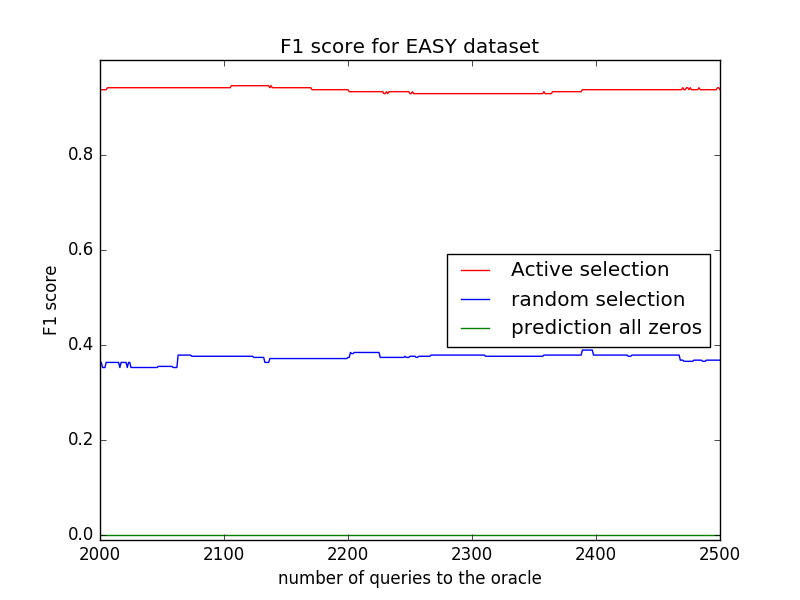
\includegraphics[scale = 0.5]{figures/f1_easy.png}
      \caption{F1 Score of easy data set plotted against number of queries made to oracle.}
      \label{easyf}
\end{figure}



\FloatBarrier
\subsection{Moderate}

\begin{figure}[!htb]
  \centering
  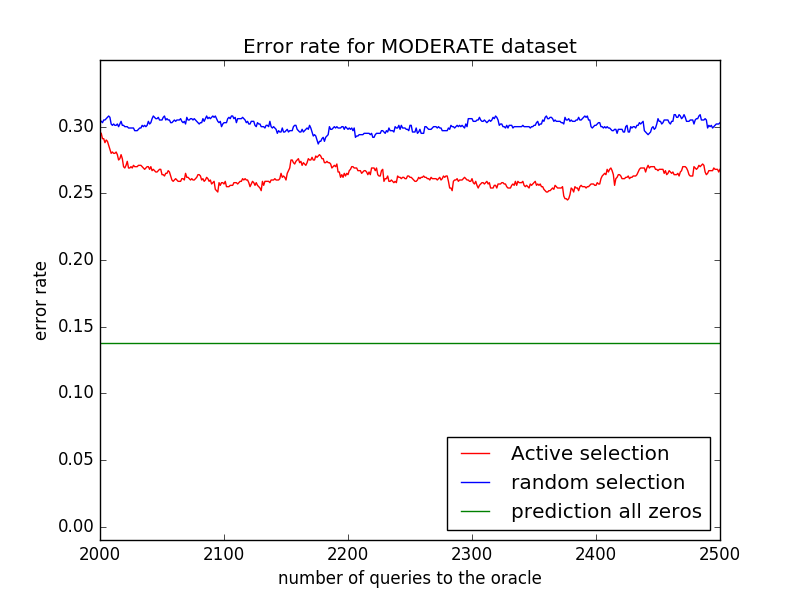
\includegraphics[scale = 0.5]{figures/error_moderate.png}
      \caption{Error rate of moderate data set plotted against number of queries made to oracle.}
      \label{moderror}
\end{figure}

\begin{figure}[!htb]
  \centering
  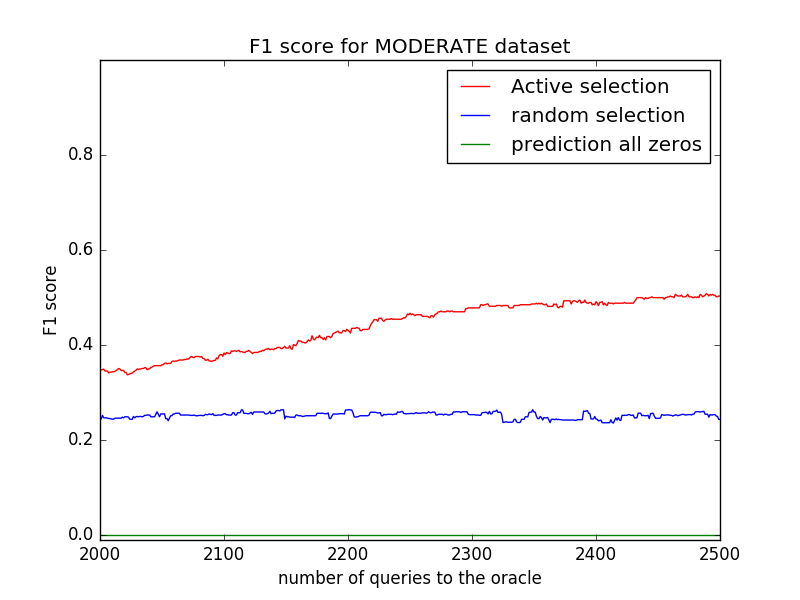
\includegraphics[scale = 0.5]{figures/f1_moderate.png}
      \caption{F1 score of moderate data set plotted against number of queries made to oracle.}
      \label{modf}
\end{figure}
\FloatBarrier
\subsection{Difficult}


\begin{figure}[!htb]
  \centering
  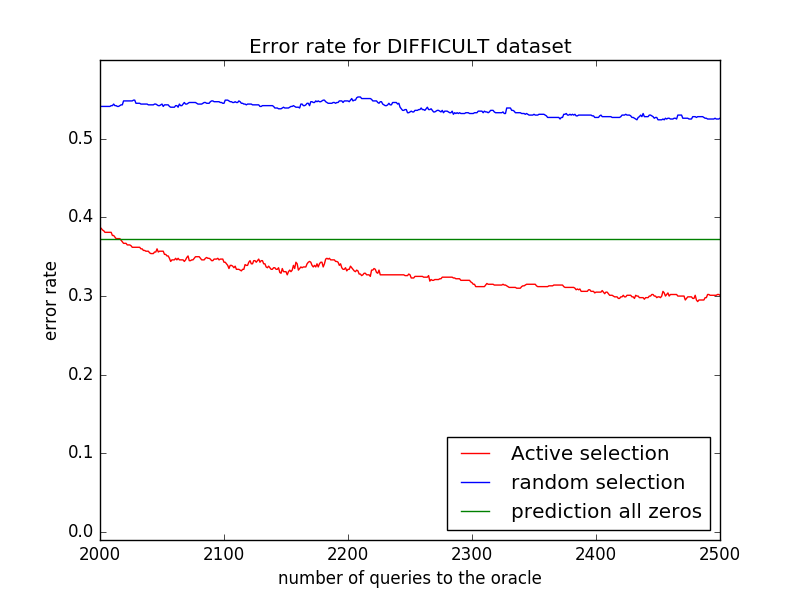
\includegraphics[scale = 0.5]{figures/error_difficult.png}
      \caption{Error rate of difficult data set plotted against number of queries made to oracle.}
      \label{harderror}
\end{figure}

\begin{figure}[!htb]
  \centering
  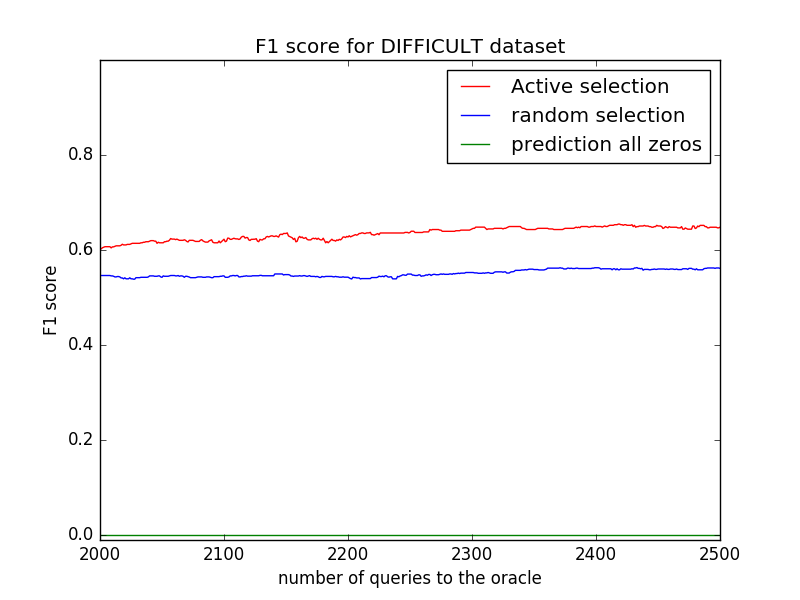
\includegraphics[scale = 0.5]{figures/f1_difficult.png}
      \caption{F1 score of difficult data set plotted against number of queries made to oracle.}
      \label{hardf}
\end{figure}

\FloatBarrier

\begin{minipage}{\linewidth}
\smallskip
\centering
\captionof{table}{F1 score of different level of test data} \label{f1table} 
\begin{tabular}{ p{2in} C{.85in} *4{C{.7in}}}\toprule[1.5pt]
\# of queries - Initial Learning & 500 & 1000 & 1500 & 2000  \\ \toprule[1.5pt]
\# of queries - Active Learning & 2000 & 1500 & 1000 & 500  \\ \bottomrule[1.25pt]
EASY                        & 0.6409                             & 0.6328                              & 0.9375                              & 0.9375                              \\
MODERATE                    & 0.2625                             & 0.4365                              & 0.4686                              & 0.5034                              \\
DIFFICULT(pos. v.s. neg.)   & 0.4286                             & 0.5133                              & 0.5346                              & 0.6481\\
\bottomrule[1.25pt]
\end{tabular} \par \bigskip
F1 score for 3 different input data, with gradient of initial vs active learning query division. 
This table shows the F1 score of each test data after the model had been trained on varying number of queries for Initial Learning (feature selection) and active learning (model learning) using the appropriate training data. 
\end{minipage}
\FloatBarrier

\begin{minipage}{\linewidth}
\smallskip
\centering
\captionof{table}{Error rate of different level of test data} \label{errortable} 
\begin{tabular}{ p{2in} C{.85in} *4{C{.7in}}}\toprule[1.5pt]
\# of queries - Initial Learning & 500 & 1000 & 1500 & 2000  \\ \toprule[1.5pt]
\# of queries - Active Learning & 2000 & 1500 & 1000 & 500  \\ \bottomrule[1.25pt]
EASY                          & 0.065                              & 0.065                               & 0.014                               & 0.014                               \\
MODERATE                      & 0.191                              & 0.142                               & 0.161                               & 0.146                               \\
DIFFICULT(pos. v.s. neg.)     & 0.622                              & 0.346                               & 0.375                               & 0.301                               \\
\bottomrule[1.25pt]
\end{tabular} \par \bigskip 
Error rate for 3 different input data, with gradient of initial vs active learning query division.
This table shows the error rate of each test data after the model had been trained on varying number of queries for Initial Learning (feature selection) and active learning (model learning) using the appropriate training data. 
\end{minipage}
\FloatBarrier


\section{Conclusion}


The increase of F1 score and the decrease of error rate using the active selection strategy can be observed in most cases. For example, the F1 score for MODERATE dataset in Figure \ref{modf} begins with similar score for random learner vs active learner, but diverges until the active learner F1 score passes 0.5. In case of the error rate for DIFFICULT dataset in Figure \ref{harderror}, active learner begins with higher error rate than guessing all 0's, but eventually becomes better than all-zero guess, resulting in lower error rate and F1 score for active learner.  Although the figures are not included for the conciseness of the report, the pattern is more prevalent when fewer number of queries were spent on feature selection and more queries were conducted using active selection. However, as shown in Table \ref{f1table} and Table \ref{errortable}, dedicating sufficient number of queries on feature selection was critical for the overall performance. As a result, all the included figures were from the experiment where 2000 queries were used for initial learning and 500 were used for active learning. 

While it has been omitted from the overall results, good amount of effort was spent on applying active learning strategy directly to the data without any feature selection. However, this ignores an important pieces of domain knowledge, where only a small subset of the training data are active, false negatives are highly undesirable, and only a small subset of features are useful in predicting activity. When we modified our strategy to conform to these domain knowledge, our error rate and F1 score improved greatly. Performance decreases with added noise in data as expected. 

Our results indicates that selecting the relevant features is critical for the learning process and overall performance, by reducing the number of dimensions and therefore the hypothesis space that the active learner must explore. This results in better performance of the learner, given the limited nature of our learning setup (limited number of queries to the oracle). In a real drug-discovery setting with a known target, it is important to balance the budget between discovering relevant features (sites, residues, molecule characteristics, etc.), as well as exploring as many molecules as possible. 

In the end, pre-feature selection, coupled with \textit{largest positive score} strategy/SVM for querying and confirming the activity of molecules as potential drug targets proved to be an effective strategy, as we prioritized our resources on discovery of active molecules rather than discovery of the decision boundary for classification, reflecting the domain knowledge and end goal of the project. 


\begin{thebibliography}{1}

%\bibitem{ref:cal}
%Cohn, Atlas, Ladner, \emph{Improving  Generalization  with  Active  Learning},  Machine Learning May 1994, Volume 15, Issue 2, p 201-221

%\bibitem{ref:dhm}
%5S. Dasgupta, D. Hsu, C. Monteleoni, \emph{A general agnostic active learning algorithm}, NIPS, 2008 

%\bibitem{ref:twoface}
%S. Dasgupta, \emph{Two faces of active learning},  \texttt{http://cseweb.ucsd.edu/$\sim$dasgupta/papers/}, 2010

\bibitem{ref:warmuth}
Warmuth, Liao, Ratsch, Mathieson, Putta and Lemmen, \emph{Active Learning with Support Vector Machines in the Drug Discovery Process}, J. Chem. Inf. Comput. Sci. 2003, 43, 667-673

\end{thebibliography}


\end{document}